\documentclass[twoside,a4paper,10pt]{article}
\usepackage[top=2.54cm,bottom=2.54cm,left=2.54cm,right=2.54cm]{geometry}

\usepackage[english]{babel}
\usepackage[utf8]{inputenc}
\usepackage{amsmath}
\usepackage{graphicx}
%\usepackage[colorinlistoftodos]{todonotes}
\usepackage{url}

\usepackage[hidelinks]{hyperref}
\usepackage{tabularx}
\usepackage{placeins}
%\usepackage{ref}

%%%

\pagenumbering{arabic}
\usepackage{fancyhdr}

\pagestyle{fancy}
% Shows section number and name
\renewcommand{\sectionmark}[1]{\markright{#1}{}}
% Clear previous styles
\fancyhf{}
\fancyhead{}
\fancyhead[RO]{\thepage}
\fancyhead[LO]{\rightmark}
\fancyhead[RE]{BitTorrent Tracker: deliverable 2}
\fancyhead[LE]{\thepage}
\fancyfoot{}
% Other modifiers
%\fancyfoot[LE,RO]{\thepage}
%\fancyfoot[LO,CE]{Something}
%\fancyfoot[CO,RE]{Author Name}

\title{BitTorrent Tracker: deliverable 2\\
  Group 01}
\author{Irene Díez \and Jesus Sesma}

\begin{document}
\date{}
\maketitle

%\begin{abstract}
%Your abstract.
%\end{abstract}
\section{Package hierarchy}\label{sec:pa-hierarchy}

Our project has the following package hierarchy:

\begin{itemize}
\item \texttt{bitTorrent}: this package holds the classes related to the
  BitTorrent protocol specification; in the following deliverables of this
  project we will change them if necessary to accommodate them to our
  implementation.
  This package will also hold the classes and packages related to networking.
\item \texttt{peer}: this package contains the classes needed by the peers. 
  Since this deliverable contemplates the design of the tracker GUI and
  project skeleton it has been left empty.
\item \texttt{tracker}: this package contains the classes needed by the tracker.
  \begin{itemize}
  \item \texttt{db}: classes related to the DB management.
    \begin{itemize}
    \item \texttt{model}: classes part of the business model.
      \begin{itemize}
      \item \texttt{TrackerMember.java}: represents a member of the tracker.
      \end{itemize}
    \item \texttt{DBManager.java}: responsible for the insert, create and
      update operations.
    \end{itemize}
  \item \texttt{gui}: holds the classes related to the graphical user interface
    of the tracker.
    \begin{itemize}
    \item \texttt{CustomJTable.java}: custom table used in the application to
      give responsive behaviour to Java's default \texttt{JTable}s.
    \item \texttt{BasicInfoPanel.java}: displays general information about
      the tracker, such as the current ID of the instance, IP and port etc.
    \item \texttt{ObserverJPanel.java}: abstract class that inherits from
      \texttt{JPanel} and implements the \texttt{Observer} interface.
    \item \texttt{PeerPanel.java}: displays information about each of the
      peers the tracker has knowledge of.
    \item \texttt{TrackerPanel.java}: displays information about the tracker
      members, such as the master and all the active slaves.
    \item \texttt{TrackerGUI.java}: holds the graphical interface of the
      tracker.
    \end{itemize}
  \item \texttt{observers}: this package holds all the observers of the
    application.
    The observers are necessary since we have decided to follow the Model View
    Controller pattern, as suggested in the specification of the deliverable.
    
    \begin{itemize}
    \item \texttt{TrackerObserver.java}: abstract base class for the observers.
    \item \texttt{DBFaultToleranceObserver.java}: observer for the
      \texttt{DBFaultToleranceSys}.
    \item \texttt{FaultToleranceObserver.java}: observer for the
      \texttt{FaultToleranceSys}.
    \item \texttt{MasterElectionObserver.java}: observer for the
      \texttt{MasterElectionSys}.
    \end{itemize}
  \item \texttt{subsys}: package that holds the subsystems of the tracker.
    
    \begin{itemize}
    \item \texttt{TrackerSubsystem.java}: abstract class that represents a
      subsystem of the tracker.
    \item \texttt{cfts}: holds the classes related to the Cluster Fault
      Tolerance System.
      \begin{itemize}
      \item \texttt{FaultToleranceSys.java}: component in charge of
        sending/receiving KA messages from the tracker members.
      \item \texttt{IpIdTable.java}: class that holds the current state of the
        cluster members.
      \end{itemize}
    \item \texttt{db}: holds the classes related to the DB fault tolerance
      system.
      \begin{itemize}
      \item \texttt{DBFaultToleranceSys.java}: class in charge of maintaining
        the reliability of the DB in the cluster.
      \end{itemize}
    \item \texttt{election}
      \begin{itemize}
      \item \texttt{MasterElectionSys.java}: class in charge of doing the master
        election process.
      \end{itemize}
    \end{itemize}
  \item \texttt{Launcher.java}: program entry point. 
  \end{itemize}
\end{itemize}

\section{Responsive design}

The tracker's gui follows the guidelines given by the responsive web design
paradigm, thereby the application's main window size and its components' size
can be adapted to a variety of screen sizes.
Figures~\ref{fig:resp-small} and~\ref{fig:resp-maxi} show an example of this
behaviour.

\begin{figure}[h]
  \centering
  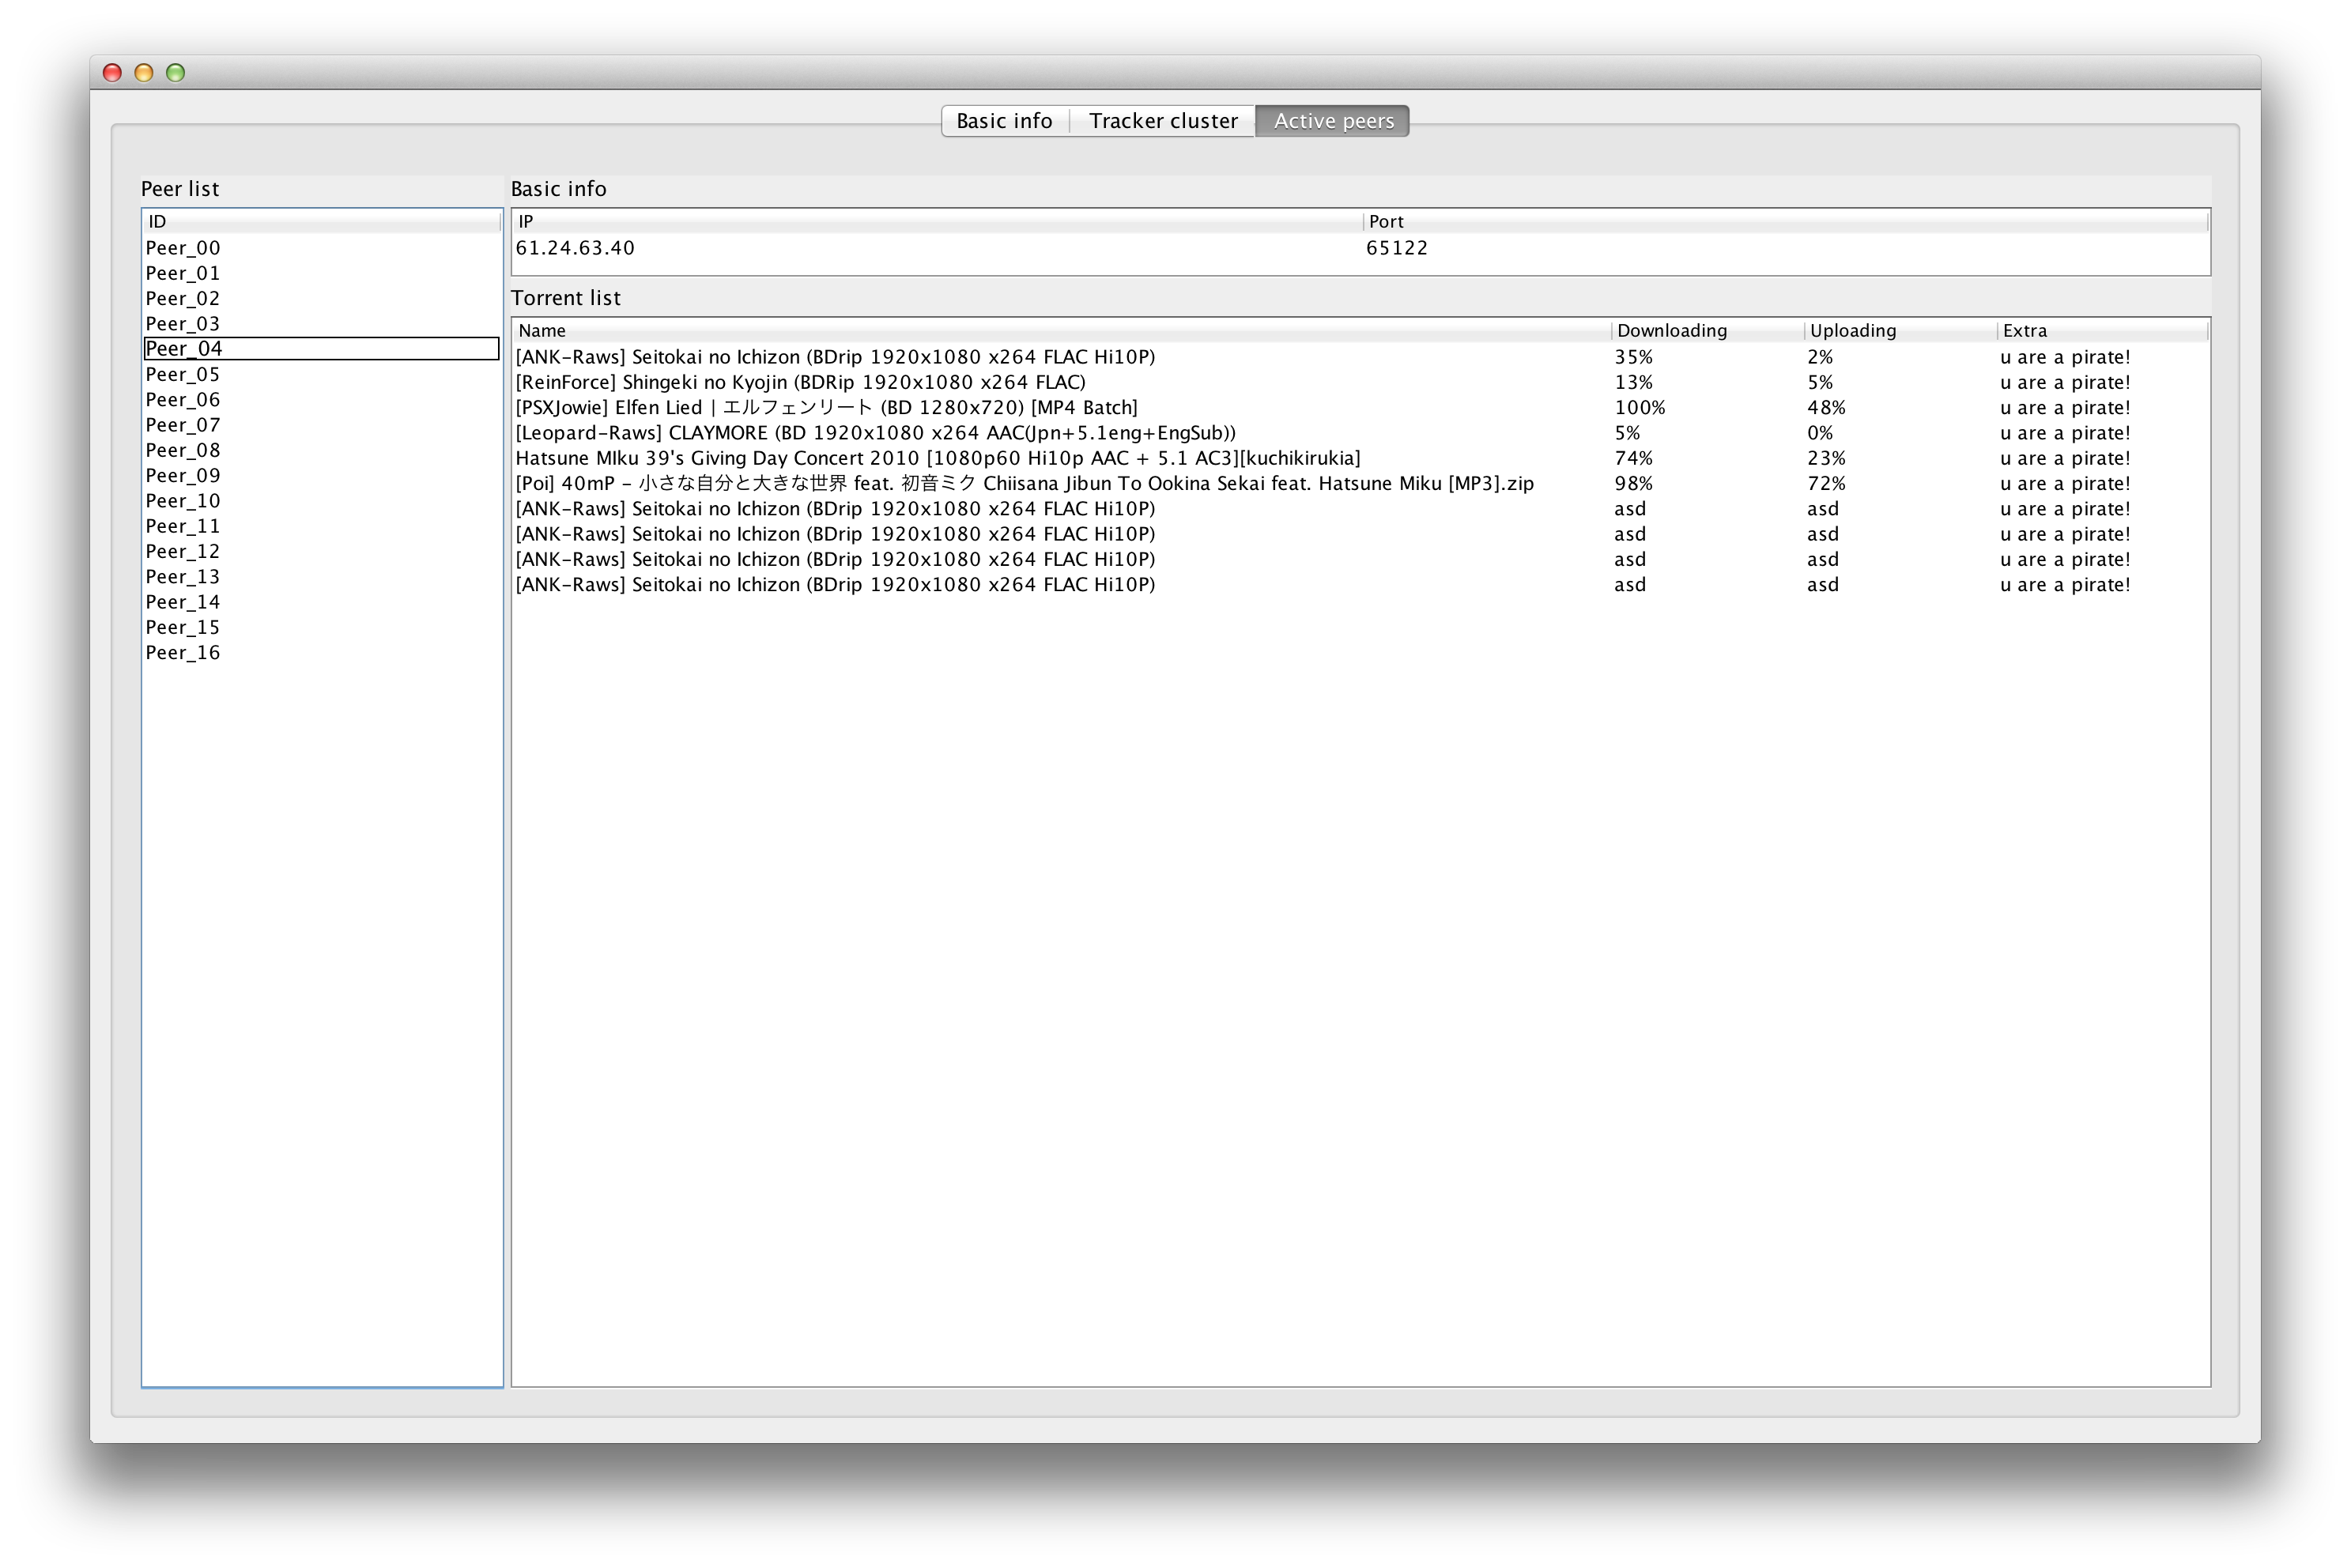
\includegraphics[width=\textwidth]{imgs/responsive_design_maximized.png}
  \caption{\label{fig:resp-maxi}Responsive behaviour: maximised window.}
\end{figure}

\begin{figure}[h]
  \centering
  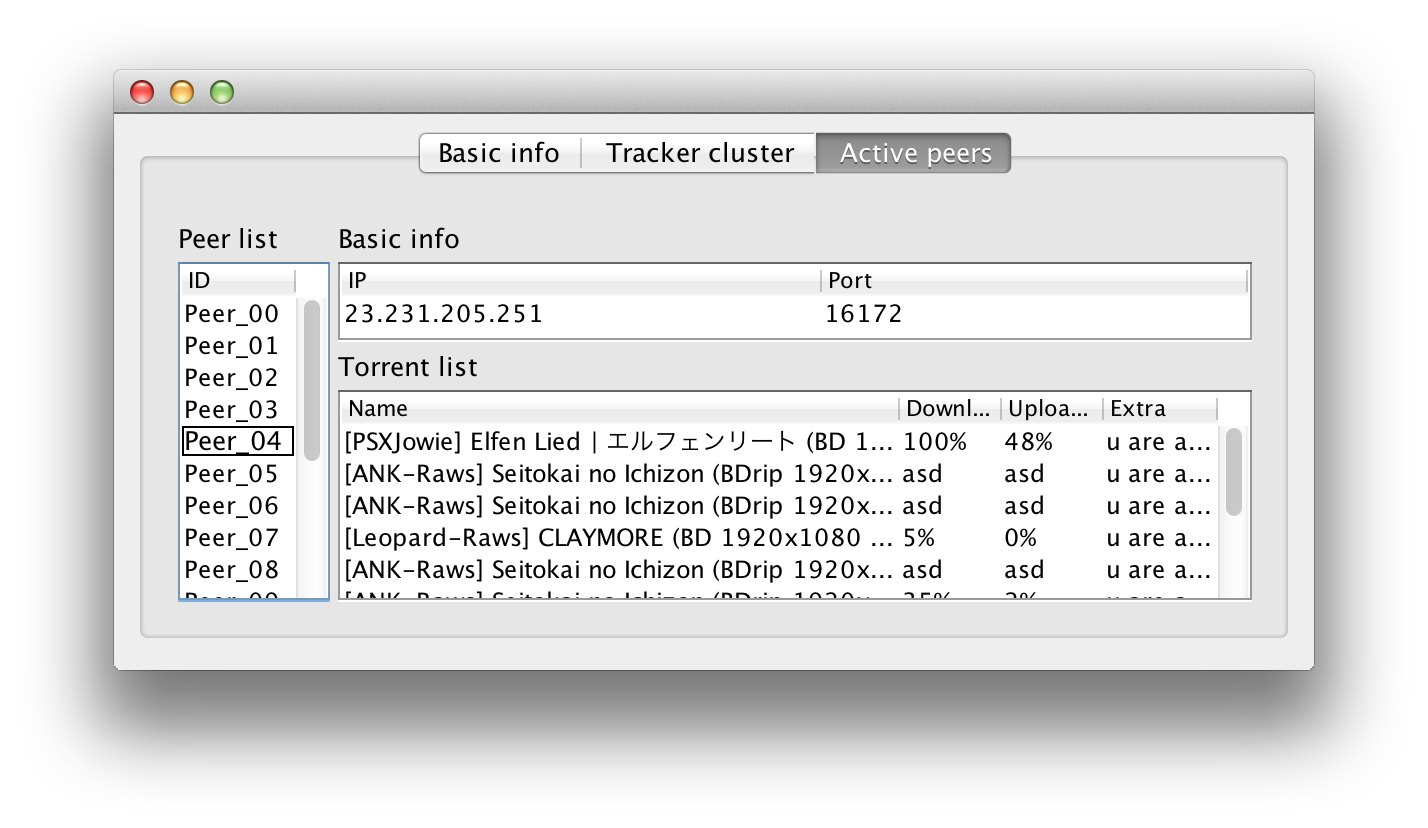
\includegraphics[width=\textwidth]{imgs/responsive_design.png}
  \caption{\label{fig:resp-small}Responsive behaviour: small window.}
\end{figure}

\section{Form validation}

Our application needs some input typed by the users, consequently that input
must be validated; and when an error is found, the user needs to be correctly
informed. Figure~\ref{fig:validation}
shows the validation and error notification of a window of the tracker.

\begin{figure}[h]
  \centering
  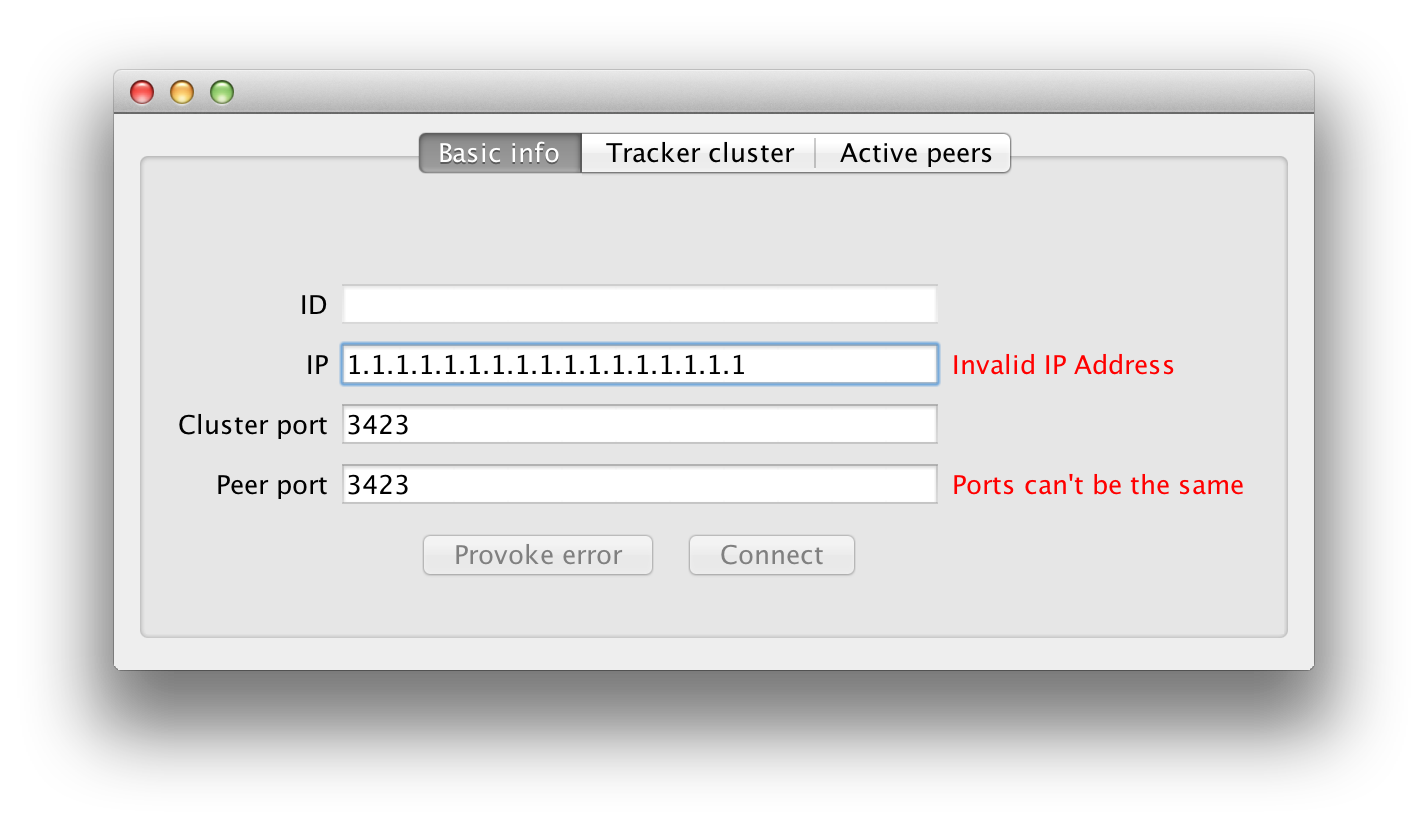
\includegraphics[width=\textwidth]{imgs/form_validation.png}
  \caption{\label{fig:validation}Forms of the \emph{Basic info} tab show
    error messages.}
\end{figure}


\section{Exception management}

Our application has a well-defined exception hierarchy previously described
in section~\ref{sec:pa-hierarchy}, please refer to this section.

%\bibliographystyle{unsrt}
%\bibliography{bib}

\end{document}


